
% This is based on the LLNCS.DEM the demonstration file of
% the LaTeX macro package from Springer-Verlag
% for Lecture Notes in Computer Science,
% version 2.4 for LaTeX2e as of 16. April 2010
%
% See http://www.springer.com/computer/lncs/lncs+authors?SGWID=0-40209-0-0-0
% for the full guidelines.
% \title{Sistemas Operacionais para Ambiente de Nuvem Computacional}
\documentclass{llncs}

\usepackage[utf8]{inputenc}
\usepackage{authblk}
\usepackage[english,portuguese]{babel}
\usepackage{graphicx}

\begin{document}

\title{Sistemas Operacionais para Ambiente de Nuvem Computacional}
%
\titlerunning{tema}  % abbreviated title (for running head)
%                                     also used for the TOC unless
%                                     \toctitle is used
%
% \author{Flávio Freitas de Sousa\and Victor Ishii}
%
\authorrunning{Flávio Freitas de Sousa and Victor Ishii.} % abbreviated author list (for running head)
%

\author[1]{Flávio Freitas de Sousa}
\author[2]{Victor Ishii}
\affil[1]{flaviofreitas.h@gmail.com}
\affil[2]{ishii.v.4@gmail.com}

%%%% list of authors for the TOC (use if author list has to be modified)
\tocauthor{Flávio and Victor Ishii}
%
\institute{Universidade Federal do Ceará, Fortaleza - CE, Brasil}

\maketitle              % typeset the title of the contribution


% ======================================================================
%   ENGLISH ABSTRACT
% ======================================================================
\selectlanguage{english}
\begin{abstract}
Since the rise in popularity of cloud computing (and its feature of treating software as a service), we witness the birth of a myriad of unavoidable questions related to the management of this kind of infrastructure. From the developer's point of view, which consumes this service from a provider, there is a strong need for softwares capable of managing access to resources, abstracting it from low-level concepts, that is, there is a huge demand for an \emph{Operational System} able to present a cloud as if it were a \emph{single} machine only, but a machine provided with a virtually unlimited amount of resources.

This paper gathers the main principles about the field of study involving the intersection between Operational Systems and Cloud Computing.
\keywords{Operational System, Cloud Computing}
\end{abstract}
\selectlanguage{portuguese}


% ======================================================================
%   RESUMO PORTUGUES
% ======================================================================
\selectlanguage{portuguese}
\begin{abstract}
Após a popularização das nuvens computacionais (e de sua característica de tratamento do software como um serviço), sugiu uma miríade de novos problemas indispensáveis relativos à gerência desse tipo de infra-estrutura. Do ponto de vista do desenvolvedor, que consome esse serviço de um provedor, existe uma forte carência de softwares capazes de gerenciar o acesso aos recursos, abstraindo seus conceitos de baixo nível, isto é, há uma grande demanda por um \emph{Sistema Operacional} que apresente a nuvem como se ela fosse uma \emph{única} máquina apenas, mas uma máquina munida de uma quantidade de recursos virtualmente ilimitada.

Este artigo reúne os principais conceitos sobre o campo de estudo que engloba a interseção entre Sistemas Operacionais e Nuvem Computacional.\\
\\
\textbf{Palavras-chave: }{Sistema Operacional, Computação em Nuvem, Nuvem Computacional}
\\[2cm]
\end{abstract}


% ======================================================================
%   OLD
% ======================================================================
% Sistemas Operacionais para Ambiente de Nuvem Computacional é um tipo de sistema operacional que opera dentro da nuvem. Com o uso da computação em nuvem o computador, tudo gera genrenciado usando a nuvem, como armazenar arquivos e fornecer os comandos de controle da máquina.Todo processamento e armazenamento será efetuado em nuvem.
% ======================================================================

% Neste artigo iremos explicar sobre os principais conceitos sobre sistema operacional em nuvem e quais são seus problemas e soluções.


% ======================================================================
%   1. INTRODUÇÃO
% ======================================================================
\section{Introdução}
Softwares distintos exigem arquiteturas distintas. Aplicações mais elementares (como uma calculadora básica), e até mesmo algumas de médio porte (como programas de edição audiovisual) necessitam de apenas uma máquina (ou algumas máquinas) para rodar. Entretanto, o crescente nível de complexidade dos serviços demandados pelos usuários gerou também nos desenvolvedores uma demanda que os afasta do gerenciamento de hardware. Consequentemente, este passa a ser um serviço "terceirizado" de larga escala. Algumas das principais causas disso são$^{[1]}$:
\begin{itemize}
\item Economia significativa na compra e manufatura de uma quantidade massiva de peças de hardware.
\item Redução notável em custos de energia e resfriamento.
\item Avanços de hardware que tornaram o uso de técnicas de virtualização de sistema viáveis e atrativas.
\item Interesse comercial crescente por um conjunto de aplicações que possam ser "carregadas na Nuvem".
\end{itemize}

A Nuvem é, então, uma abstração para uma \emph{mega estrutura} de servidores distribuídos cujo acesso é alugado e alocado de forma dinâmica, isto é, mediante requisições dos clientes, que podem ser automatizadas e não necessitar diretamente da autorização de um humano.

Assim, uso de hardware torna-se um serviço, bem como o próprio uso de software. Esse \emph{modus operandi} remete bastante à forma como é feita a distribuição de energia elétrica. O cliente utiliza a quantidade que desejar ao longo do mês, sem necessidade de requisições formais à companhia de energia para acender uma lâmpada ou ativar um microondas. O uso é contabilizado ao longo do mês, e o cliente recebe uma conta mensal. Do mesmo modo, o desenvolvedor escolhe uma empresa que oferte serviços de \emph{back-end} de Nuvem, e começa a desenvolver seu software segundo a interface da distribuidora, que permitirá a alocação dinâmica de máquinas a partir do código do software produzido pelo desenvolvedor. Este, então, será taxado mediante diversos fatores, como quantidade de máquinas alocadas, tempo de uso, qualidade do hardware etc.

Por conseguinte, na integração com a Nuvem, o desenvolvedor torna-se responsável por diversas tarefas de comunicação e gerenciamento semelhantes aos problemas tratados por um sistema operacional comum. Isso ocorre por que ela não é uma máquina única, e não há um sistema operacional que a gerencie. Contudo, o tratamento desses problemas não é interessante para o desenvolvedor, e, portanto, pesquisas recentes buscam o desenvolvimento de sistemas operacionais robustos, que atuem como uma interface entre o desenvolvedor e a Nuvem, apresentando-a não como um conjunto de máquinas a ser gerenciado por software, mas como se fosse uma máquina única com uma quantidade de recursos colossal.

% ======================================================================
%   2. ARQUITETURA
% ======================================================================
\section{Arquitetura}
Nesta seção vamos mostrar como funciona a arquitetura do sistema operacional em nuvem.$^{[1]}$

\begin{center}
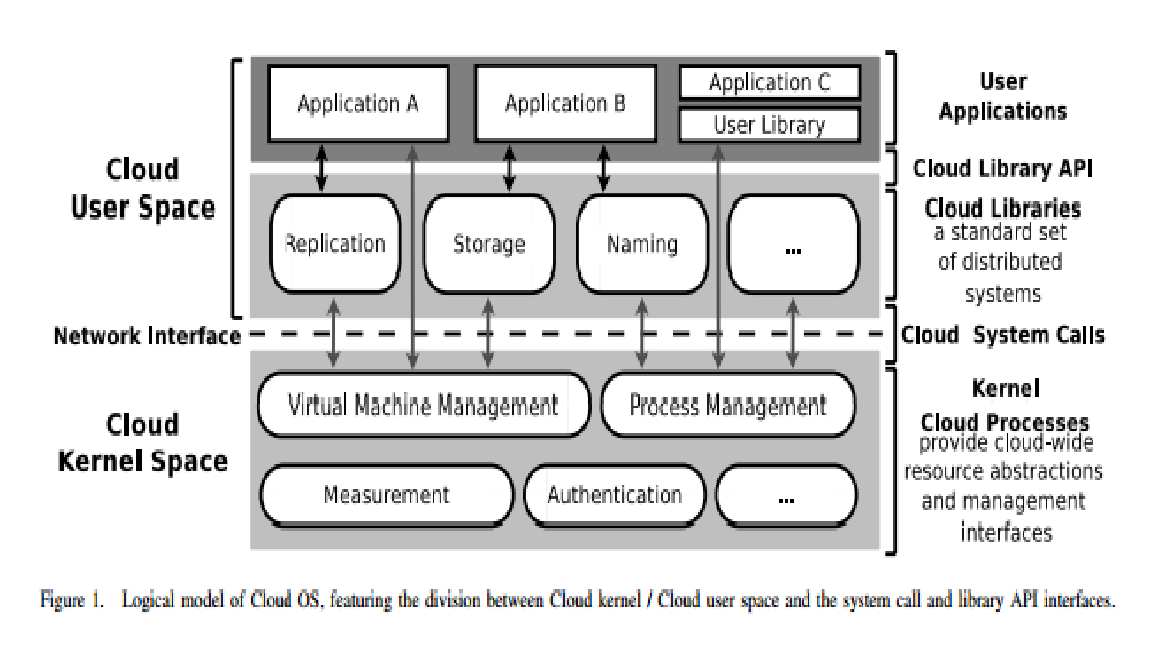
\includegraphics[width=12cm]{arq.png}
\end{center}

% 2.1. Arquitetura lógica ------------------------------------
\subsection{Arquitetura lógica do sistema operacional em nuvem}
Figure 1 representa o modelo lógico da computação em nuvem. Nós definimos um objeto em nuvem como um conjunto local de processos do sistema operacional que está em execução em um único nó, cujo estão entrelaçados e associados localmente com um identificador aleatório de tamanho adequado pra minimizar os riscos de colisões dos identificadores.

É referido para o pequeno número de processos na nuvem que regulam alocação física, controle de acesso e medidas dos recursos como espaço do kernel na nuvem. Processo que são executados diretamente pelo usuário são chamados de aplicação de usuário, enquanto biblioteca na nuvem são processos na nuvem tipicamente chamados pelas aplicações e outras bibliotecas. Aplicações podem interagir com as bibliotecas e os processos do kernel na nuvem pela rede através de um conjunto de interfaces padrões chamados chamadas de sistemas na nuvem. Basicamente a havilidade de executar processos do kernel na nuvem, junto com a disponibilidade de apropriadas credenciais de segurança, é uma condição suficiente para o nó fazer parte da nuvem.

Todos os objetos no espaço do usuário na nuvem podem ser acessados  pela rede. A associação entre nomes dos objetos e seus endereços na rede e portas é gerenciado pelo gerenciamento de processos e gerenciador da máquina virtual e o resultado dessas informações é disponibilizado pela nuvem através da biblioteca de nomes. Essa biblioteca também mantém atualizado a localização das conexões entre os processos na nuvem do espaço do usuário e os objetos dos quais eles são compostos. Os direitos de acessos necessários para todas essas operações de gerenciamento são garantidos e verificados pera autentificação dos processos do kernel na nuvem.

% 2.2. Kernel process ------------------------------------
\subsection{Implementação dos processos do kernel na nuvem}

\begin{enumerate}
\item \emph{Medidas de recursos} \\
O sistema operacional em nuvem precisa ter uma fácil visualização com os recursos da nuvem disponíveis. Isso é feito realizando medidas locais em cada nó da nuvem. \\

\item \emph{Abstrações de recursos} \\
Caracterizar a rede subjacente é uma exigência crucial para o sistema operacional em nuvem. Uma das principais vantagens na interface baseada em arquivo é que tem uma grande flexibilidade e suas desvantagens podem ser resolvidas com o apropriado uso de convenção de nomes.
\item \emph{Distribuições de processos e gerenciamento de aplicações} \\
Sistema operacional em nuvem instancia e gerencia todos os objetos que existem nos nós da nuvem. Virtualização provêm muitas propriedades requeridas no ambiente na nuvem, tais como o suporte para sistemas operacionais de múltiplas plataformas do mesmo nó e a isolação implícita entre processos que estão sendo executados em diferentes máquinas virtuais no mesmo hardware.

\item \emph{Controle de acesso e autenticação de usuário} \\
Provêm suporte integrado para grandes números de usuários que simultaneamente requerem um método de autenticação para evitar pontos de falhas, isso resulta uma completa ou parcial inacessibilidade dos recursos em nuvem.
\end{enumerate}


% 2.3. Características fornecida pelo espaço do usuário na nuvem -----------
\subsection{Características fornecida pelo espaço do usuário na nuvem }
Para aproveitar todo o potencial da nuvem, desenvolvedores devem receber acesso a um conjunto de caminhos padrões para satisfazer requerimentos comuns de aplicações de distribuição de alta escala. Biblioteca em nuvem disponibiliza de uma interface de programação de aplicativos padrão com as seguintes características:  
\begin{itemize}
\item Acesso aos objetos na nuvem e nomes dos processos pelo DNS e/ou outros serviços.
\item Funcionalidade de armazenamento confiável distribuída.
\item Implantação automatizada de aplicativos em nuvem, escalonamento horizontal e gerenciamento do ciclo de vida.
\item Grande suporte da disponibilidade de failover com execução de processos replicados com checkpoints.

\end{itemize}
% ======================================================================
%   3. TRABALHOS RELACIONADOS
% ======================================================================
\section{Resumo dos Trabalhos Relacionados}


% 3.1. Definições ------------------------------------
\subsection{Definições}
\quad Esta seção possui uma lista com as definições mais relevantes encontradas em diversos artigos.

\begin{itemize}
\item \textbf{Node \cite{pia}} \\
Um \emph{nó} é uma máquina da nuvem, uma peça de hardware a nível de consumidor básico; uma parte comum e não custosa.\\

\item \textbf{Cluster \cite{pia}} \\
Um conjunto de nós que pertencem à mesma instalação.\\

\item \textbf{Cloud Object \cite{pia}} \\
Um \emph{Objeto em Nuvem} é definido como um conjunto local de processos de sistema operacional que rodam em um único nó. \\

\item \textbf{Cloud Process \cite{pia}} \\
\emph{Processo em Nuvem} é uma coleção de Objetos em Nuvem que implementam a mesma aplicação (geralmente distribuída). \\

\end{itemize}


% 3.2. Desafios ------------------------------------
\subsection{Desafios \cite{wentz}}
\begin{itemize}
\item \textbf{Escalabilidade} \\
Os sistemas operacionais tradicionais foram projetados para processamentos batch. Apenas recentemente, com a ascensão do processamento paralelo, máquinas com maiores quantidades de núcleos tem se popularizado.

Nesse contexto, a Computação em Nuvem apresenta demandas extremamente flexíveis (e até impresivíseis). Além disso, os modelos de serviços das Nuvens eliminam a limitação de escalabilidade por hardware, substituindo-a por uma limitação monetária. Tudo isso leva a escalabilidade à uma posição de fator vital no projeto de sistemas em Nuvem. \\

\item \textbf{Variabilidade de Demanda} \\
\emph{Elasticidade}, ou variabilidade de demanda, é outro fator a ser inevitavelmente gerenciado. Na maioria dos casos, a quantidade de clientes acessando o serviço em função do tempo não obedece padrões bem comportados. Ao contrário, diversos são os picos e gargalos, nos quais uma grande parte da base de usuários (80\% ou mais) decide consumir o serviço simultaneamente durante um curto intervalo de tempo, bem como são frequentes os longos periodos de ociosidade que intercalam esses picos. Um sistema para Nuvem deve gerenciar a quantidade de máquinas ativas de forma escalável, ao passo que um sistema tradicional apenas gerencia se um núcleo está (ou alguns poucos núcleos estão) ativo(s) ou ocioso(s). \\

\item \textbf{Tolerância a Falhas} \\
A indústria de hardware tem constantemente diminuído o tamanho dos transistores e aumentado sua contagem em cada chip. Consequentemente, a probabilidade de erros ocorrerem é também amplificada. Por isso, os sistemas mais novos começam a considerar o tratamento de falhas como uma preocupação relevante.

No contexto das Nuvens, falhas são muito mais propensas, posto que esse ambiente é ainda mais distribuído e muitas vezes apresenta vários usuários que competem pelos mesmos serviços e trabalham em cima dos mesmos arquivos. \\

\item \textbf{Programação} \\
O desenvolvimento de aplicativos dentro dessa realidade apresenta sérios desafios de programação, uma vez que se faz necessário o uso extensivo de programação concorrente. Sistemas operacionais baseados na estratégia tradicional de \textbf{locking} são difíceis e propensos a erros.

Além disso, o modelo de \emph{infraestrutura como um serviço (IaaS)} adiciona um nível extra a ser tratado devido à utilização de máquinas virtuais. Outra tarefa complexa é o \textbf{balanceamento de carga}, que tenta impedir que o sistema atinja estados que aprensentem nós sobrecarregados e nós livres simultaneamente, distribuindo as tarefas igualmente, na medida do possível.

\end{itemize}


% 3.3. Desafios ------------------------------------
\subsection{Requerimentos de um S.O. em Nuvem \cite{pia}}
Um sistema operacional em Nuvem deve:
\begin{enumerate}
\item \emph{Permitir o gerenciamento autônomo de seus recursos por parte de seus usuários e aplicações.} \\
Considerando a alta variabilidade de demanda, os usuários devem ser capazes de alocar em tempo real e de forma flexível os recursos a serem utilizados. Na nossa analogia com o modelo de distribuição elétrica, isso equivale a não deixar um eletrodoméstico consumindo energia desnecessariamente. Recursos alocados inconsequentemente serão tarifados sem necessidade e, além disso, poderiam ser realocados para outro usuário que estivesse, de fato, fazendo uso desses produtos. \\

\item \emph{Continuar funcionando mesmo após uma perda de nós, de clusters, ou uma partição de rede}.
Pela \\
Os componentes de um sistema em nuvem estão sempre sujeitos a falhas parciais ou totais, temporárias ou permanentes, e o sistema deve estar preparado para isso. O sistema deve resolver seus problemas internos sem a necessidade de contactar o usuário, que deve continuar usufruindo dos serviços normalmente, como se não existissem falhas. \\

\item \emph{Ser independente dos sistemas operacionais envolvidos e agnóstico à arquitetura.} \\
Os serviços devem ser fornecidos por meio de uma interface padronizada, que deve ser independente de qual sistema operacional ou arquitetura o cliente esteja se comunicando. \\

\item \emph{Suportar múltiplos tipos de aplicações, incluindo as legadas.} \\
A retrocompatibilidade é um fator bastante relevante nesse cenário. Devido à grande abrangência de serviços da Nuvem, ela também deve ofertar compatibilidade com sistemas e aplicações legados, e consequentemente, nosso sistema deve oferecer essa possibilidade.\\

\item \emph{Ser descentralizado, escalável, ter pouco overhead por usuário e por máquina, e ser efetivo em custo.} \\
Essas são características já esperadas de um software usável. A descentralização é importante no contexto da Nuvem, pois um sistema centralizado vai de encontro ao propósito distribuído desse cenário, minando a disponibilidade e a tolerância a erros do ambiente de Nuvem.\\

\item \emph{Ser contabilizável em termos de recursos utilizados.} \\
Como estamos lidando com um serviço a ser provido e taxado mediante o uso, é preciso que haja um meio confiável de contabilização do consumo dos clientes. \\

\end{enumerate}

% ======================================================================
%   4. PROBLEMAS
% ======================================================================
\section{Descrição do Problema}
Escalabilidade, variabilidade de demanda, tolerância a falhas e dificuldade na programação de sistemas grandes são os desafios mais comuns de sistemas em nuvem.

Existem muitas questões fundamentais ainda sem respostas \cite{nurmi}: 
\begin{itemize}
\item Qual é a melhor arquitetura para sistemas computacionais em nuvem?
\item Quais características de recursos o cronograma de instância da máquina virtual deve considerar para utilizar os recursos de maneira mais eficiente?
\item Como podemos construir redes de instância da máquina virtual que são flexíveis, de alto desempenho e seguras? 
\item  quais domínios de aplicação mais se beneficiam com o sistema operacional em nuvem e quais interfaces são apropriadas? 
\item  Quais tipos de acordo de nível de serviço a computação em nuvem disponibiliza?
\item  Como sistemas operacionais em nuvem podem se associar com mais recursos comuns providos pelos sistemas já disponíveis?
\end{itemize}

Sistemas de computação em nuvem fornecem uma vasta variedade de interfaces e abstrações desde da habilidade de dinamicamente preparar máquinas virtuais até fornecer um acesso flexível para os serviços de software.

Por exemplo, para o usuário construir uma aplicação que possa conseguir uma vantagem de mais de uma única maquina virtual, a aplicação do usuários precisa reconhecer o que ela precisa, comunica suas necessidades para o gerente da nuvem, e gerência a comunicação entre as máquinas.\cite{wentz}

A escalabilidade na nuvem tem um preço. Ele precisa realizar trocas com outras propriedades de sistemas requeridos. Pelo fato da nuvem ser acessada pro milhares de pessoas, ela precisará ser bastante escalável e sempre disponível.\cite{liu}

% ======================================================================
%   5. SOLUÇÃO
% ======================================================================
\section{Descrição da Solução}
Abaixo listamos algumas das soluções mais citadas para os diversos problemas encontrados:

\begin{enumerate}
\item \emph{Desafio relacionado a escalabilidade: Escalabilidade horizontal.} \\
Quando usado o SimpleDB, sistema de banco de dados na nuvem da Amazon, cada domínio só consegue suportar uma pequena taxa de entrada. Para resolver esse problema deverá ser necessário espalhar as instruções de entrada por diversos domínios e depois será agregado todos os resultados de todos os domínios quando for pedido o seu estado.\cite{liu} \\

\item \emph{Desafio relacionado a variabilidade de demanda: Mensagens duplicadas.} \\
Quando uma thread ler uma mensagem na fila, a mensagem desaparece da fila por um certo tempo. Caso duas threads acessem a mesma mensagem, elas podem ler a mesma mensagem duas vezes. Para resolver esse problema é utilizado técnicas de MapReduce na nuvem.\cite{liu} \\

\item \emph{Desafio relacionado a tolerância a falhas: Latência alta.} \\
Como os serviços são acessados pela rede é natural se esperar uma grande latência, um atraso nas instruções. É possível resolver esse problema através de duas técnicas: agregação de mensagens e multi-threading.\cite{liu} \\

\item \emph{Desafio relacionado a programação: Potencial falha dos nó.} \\
Uma thread pode falhar no meio da tarefa. Para resolver esse problema é utilizado uma atualização de estado, isso irá acompanhar o estado das threads, caso seja encontrado um resultado não salvo, ele será removido. \\
\end{enumerate}

% ======================================================================
%   6. CONCLUSÃO
% ======================================================================
\section{Conclusão}
A existência de uma simples, poderosa e expressiva abstração é essencial para alcançar todo o potencial da Computação em Nuvem. Mas devido à heterogeneidade desse meio, tal sistema deve implementar toda uma gama de técnicas para que consiga satisfazer a notável pluralidade de problemas advindos desse contexto, apresentando uma solução diferenciada para cada problema.

Por fim, este artigo observa os principais pontos referentes a sistemas operacionais em Nuvem, analisando arquitetura, desafios e vantagens.

% ======================================================================
%   REFERÊNCIAS
% ======================================================================
\begin{thebibliography}{5}
%
\bibitem {pia}
Pianese, F., Bosch, P., Duminuco, A., Janssens, N., Stathopoulos, T., Steiner, M.:
Toward a Cloud Operating System., 
Network Operations and Management Symposium Workshops (NOMS Wksps), 2010.

\bibitem {wentz}
Wentzlaff, D. , Gruenwald III, C., Beckmann, N., Modzelewski, K., Belay A., Youseff, L., Miller, J., Agarwal, A.:
An Operating System for Multicore and Clouds: Mechanisms and Implementation. Cambridge, MA 02139, 2010.

\bibitem {nurmi}
Nurmi, D., Wolski, R., Grzegorczyk, C., Obertelli, G., Soman, S., Youseff, L. E Zagorodnov, D.
Eucalyptus: an open-source cloud computing infrastructure. 
Journal of Physics: Conference Series, v. 180, p. 012051, 2009.

\bibitem{smets}
Smets-Solanes, J., Cerin, C., Courteaud, R., 
SlapOS: a Multi-purpose Distributed Cloud Operating System Based on an ERP Billing Model, 
IEEE, 2011.

\bibitem{liu}
Liu, H., Orban, D.,
Cloud MapReduce: a MapReduce Implementation on top of a Cloud Operating System.,
2011 11th IEEE/ACM International Symposium on Cluster, Cloud and Grid Computing.
% \bibitem{armbr}
% Armbrust, M., Fox, A., Griffith, R., Joseph, A. D., Katz, R. H., Konwin-ski, A., Lee, G., Patterson, 
% D. A., Rabkin, A., Stoica, I., and Zaharia, M. (2009). 
% Above the clouds: A berkeley view of cloud computing. Technical report, EECS Department, University of California, Berkeley.





% \bibitem {clar:eke:2}
% Clarke, F., Ekeland, I.:
% Solutions p\'{e}riodiques, du
% p\'{e}riode donn\'{e}e, des \'{e}quations hamiltoniennes.
% Note CRAS Paris 287, 1013--1015 (1978)

% \bibitem {mich:tar}
% Michalek, R., Tarantello, G.:
% Subharmonic solutions with prescribed minimal
% period for nonautonomous Hamiltonian systems.
% J. Diff. Eq. 72, 28--55 (1988)

% \bibitem {tar}
% Tarantello, G.:
% Subharmonic solutions for Hamiltonian
% systems via a $\bbbz_{p}$ pseudoindex theory.
% Annali di Matematica Pura (to appear)

% \bibitem {rab}
% Rabinowitz, P.:
% On subharmonic solutions of a Hamiltonian system.
% Comm. Pure Appl. Math. 33, 609--633 (1980)

\end{thebibliography}

\end{document}
